% Run
% xelatex "\def\ishandout{1} \input{../lecture-header}

\LuaCodeDebugOn
\luaexec{dofile("src/graph.lua")}

\begin{document}
\documentclass[12pt,a4paper]{article}
\usepackage{listings}

\def\algorithm#1{{\noindent\bf Algorithm #1.~}}
% some listings definitions for MMIX language
\def\lstmmix{
  \lstset{
    frame=single,
    numbers=left, 
    numberstyle=\tiny,
    numbersep=5pt,
    tabsize=4,
    sensitive=true,
    columns=fixed,
    morekeywords={ADD,ADDU,BN,BNN,BNP,BNZ,BYTE,BZ,CMP,GETA,GREG,
      IS,JMP,LDO,LDOU,LOC,
      NEG,OCTA,PBN,PBNZ,PBZ,POP,SET,SL,STO,STOU,TRAP},%added
                                %on demand
    morecomment=[l]{*},
    columns=flexible,
    commentstyle=\scriptsize,
    escapechar={\%,\#}}}
% some listings definitions for MIPS language
\def\lstmips{
  \lstset{numbers=left, 
    numberstyle=\tiny,
    numbersep=5pt,
    tabsize=5,
    morekeywords={add,addi,beq,bne,jal,jr,la,lb,li,lw,move,sll,slt,sw,syscall},
    columns=flexible,
    morecomment=[l]{\#},
    commentstyle=\scriptsize
  }}

\begin{document}

\section*{\hfil Preface}

\bigskip

Some algorithms of sorting and seaching are studied. Most of them are
based on that showed in Don Knuth's ``The Art of Computer
Programming'' volume 3. The algorithms are implemented in MMIX
assembly language as a straight translation of MIX version.

Some algorithms are implemented in MIPS assembly language to study how
differents characteristics of different processors can affect the
algorithm. In the MIPS implementations the algorithms are implemented
as subroutines to facilitates the tests calling them on other pieces
of code. Another difference when compared to MMIX implementation is
that the array index starts at zero, fitting better with the
instructions provided by the language.

Some algorithms are specified using TLA+ language to study the formal
relations between the elements of them.

\section{Searching}

\subsection{Sequential searching}

The sequential search is the most straightfoward method of search, and
for this reason its complexity time when compared to other search
algorithms is expensive.

The MMIX implementation follows almost exactly the steps stated by
Prof. Donald Knuth in the ``Art of Computer Programming'' volume 3,
page 396. The only modification and this modification will be carried
throughout this manuscript is that algorithm is implemented as a
function. 

In the S algorithm {\tt \$0} is the return value, and is the index of
the array to search for key, if the key is found, otherwise is
-1. Unsing the index the information can be retrieved from {\tt
  INFO[i]}. The rest of the registers are {\tt K[i]} $\leftarrow$ {\tt
\$1}, {\tt N} $\leftarrow$ {\tt \$2}, and the temporary registers {\tt
K[i]} $\leftarrow$ {\tt \$254} and {\tt t} $\leftarrow$ {\tt \$255}.


\algorithm{S}

\lstmmix
\lstset{
  caption={MMIX implementation of algorithm S.},
  label={mmix:s}
}
\lstinputlisting{search/sequencial.mms} % Program S

The analysis depends on two things,
\begin{center}
  C = the number of comparisons;\\
  S = 1 if successful, 0 if unsuccessful.
\end{center}

The way program S was implement, it takes $6C-S+3$ units of time. When
the search is successful, $C=i$, $S=1$ and runing time is $(6i+2)u$,
when the search fails, $C=N$, $S=0$ and running time is $(6N+3)u$.


In the MIPS implementation of algorithm S (Listing~\ref{mips:s}), the
argument register {\tt \$a0} contains the base address of $K_i$, and
{\tt \$a1} the number $N$ of array elements and {\tt \$a2} contains
the value of $K$. The function {\tt S(K[i], N, K)} returns {\tt -1} if
the key is not found and the index {\tt i} of the key to the caller
get {\tt INFO[i]}, the corresponding to the information associated
with the key.

\lstmips
\lstset{
  caption={MIPS implementation of algorithm S.},
  label={mips:s}
}
\lstinputlisting{search/sequencial.s} % Program S

\algorithm{Q}
The idea of algorithm $Q$ is similar to $S$, the only and important
difference is that a key is added at $N+1$ containing the value of $K$
associated. This trick frees the need to verify if the array has
reached the end inside the loop. This condition is verified after
using the fake new element at the end of array.

\lstmmix
\lstset{
  caption={MMIX implementation of algorithm Q.},
  label={mmix:q}
}
\lstinputlisting{search/quicksequential.mms} % Program Q

The running time of program $Q$ has decreased to $(5C+6)u$. When the
search is unsuccesfull the program $Q$ becomes faster than $S$ when
$N>3$.

\lstmips
\lstset{
  caption={MIPS implementation of algorithm Q.},
  label={mips:q}
}
\lstinputlisting{search/quicksequential.s} % Program Q


\def\curralgor{T}
\algorithm{\curralgor}
\lstmmix
\lstset{
  caption={MMIX implementation of algorithm \curralgor.},
  label={mmix:\curralgor}
}
\lstinputlisting{search/tree.mms} % Program T

The running time for searching phase (up to line 31) is
$(6C+C1-2S+2)$, where
C = number of comparisons made;\\
C1 = numer of times $K\leq KEY(P)$;\\
C2 = number of times $K>KEY(P)$;\\
S = [search is successful].

\def\lang{mips}
\lstmmix
\lstset{
  caption={\uppercase{\lang}\ implementation of algorithm \curralgor.},
  label={\lang :\curralgor}
}
\lstinputlisting{search/tree.s} % Program T

\end{document}

\end{document}
"
% to disable transitions

\ifdefined\ishandout
  \documentclass[handout]{beamer}
\else
  \documentclass[]{beamer}
\fi

\setbeamercovered{highly dynamic}
\newcounter{saveenumi}% save counter on enumerate across frames
\newcommand{\seti}{\setcounter{saveenumi}{\value{enumi}}}
\newcommand{\conti}{\setcounter{enumi}{\value{saveenumi}}}
\resetcounteronoverlays{saveenumi}

% Dependencies
\usepackage{fontspec} % use XeLaTeX
\usepackage[]{polyglossia}
\setdefaultlanguage{brazil}
% \usepackage{lcg} % Generate random numbers
\usepackage{hyperref}
\hypersetup{colorlinks=true,linkcolor=blue,anchorcolor=blue,urlcolor=blue}
\usepackage{pgf,tikz} % Draw figures
\usetikzlibrary{arrows,automata,calc,chains,circuits,graphs,positioning,shapes.gates.logic.US,shapes,trees}
\usepackage{circuitikz}
%\usepackage{pgfgantt}
  % \usepackage{pgfplots}
  % \usegdlibrary{trees}
  \usepackage{listings}
  \lstset{language=C,inputencoding=utf8,basicstyle=\footnotesize, 
    flexiblecolumns=true, numbers=left, numberstyle=\tiny\color{gray}, 
    commentstyle=\scriptsize\color{black!50},mathescape}
  \usepackage{pdftexcmds} % \pdf@strcmp \pdf@filemoddate
  \usepackage{ifthen} % \ifthenelse
  \usepackage{animate}

  % FONTS
  \font\fiverm=cmr5
  \font\ninerm=cmr9

  % Definitions
  \author{Adriano J. Holanda}%\\{\scriptsize \url{http://holanda.xyz}}}
  \def\array{vetor}
  \def\bigO#1{\mathcal{O}(#1)}
  \def\bug#1{{\it bug#1\/}}
  % C letter
  \font\ninerm=cmr9
  \let\mc=\ninerm
  \def\CEE{{\mc C\spacefactor1000}}

  \def\boxset{
    \tikzset{box/.style={rectangle,minimum width=.5cm,draw},
      index/.style={minimum width=.5cm}}
  }

  % only title frames
  \def\onlytitleframe#1{\author{}\date{}\title{#1}\maketitle}

  % THEOREM
  % \newtheorem{teorema}[theorem]{Teorema}

  \newcommand{\executeiffilenewer}[3]{%
    \ifnum\pdf@strcmp{\pdf@filemoddate{#1}}%
    {\pdf@filemoddate{#2}}>0%
    {\immediate\write18{#3}}\fi%
  }
  % includesvg[includegraphics args]{file} command (linux-version)
  \newcommand{\includesvg}[2][]{%
    \executeiffilenewer{#2.svg}{#2.pdf}{%
      /usr/bin/inkscape -z -C --file="#2.svg" --export-pdf="#2.pdf" > /tmp/#2.log}%
    \ifthenelse{\equal{#1}{}}{%
      \includegraphics{#2}}{%
      \includegraphics[#1]{#2}}%
  }

\def\lecturetitle#1#2{\title{{\large\bf#1}\\{\small [#2]}}}

\def\transitionslide#1{\frame{\author{}\title{\LARGE#1}\date{}\maketitle}}

  \def\shcmd#1{
    \begingroup
    \bigskip\color{gray}
    {\tt \$~#1}
    \bigskip
    \endgroup
  }


  \def\fonte#1{\begingroup\tiny\tt\color{gray} Fonte:~#1\endgroup}

\title{Grafos: terminologia e representação}

\begin{document}

\begin{frame}{Por que grafos?}

\begin{columns}
\begin{column}{0.45\textwidth}
\only<1>{\includegraphics[scale=0.45]{img/southam_map_nocolor}}
\only<2>{\includegraphics[scale=0.35]{img/southam_map_color}}
\end{column}
\begin{column}{0.55\textwidth}
\only<1>{\includegraphics[scale=0.2]{img/southam_nocolor.png}}
\only<2>{\includegraphics[scale=0.2]{img/southam_color.png}}
\begin{center}
{\footnotesize 1 -- Brasil, 11 -- Argentina}
\end{center}
\end{column}
\end{columns}

\end{frame}

\begin{frame}{Grafo: Definição}

\begin{block}{Informal}
Grafo G é formado:
\begin{itemize}
\item Conjunto finito de vértices $V$;
\item Relação simétrica $R$ em $V$ entre os pares de vértices;
\item O conjunto de pares simétricos $R$ é denotado por $E$.
\end{itemize}
\end{block}

\begin{block}{Formal}
$G = (V, E)$ \\
$\{v \in V : v \notin \emptyset\}$ \\
$\{ \{(u, v), (v, u)\} \in R : (u, v) \in E \land \{u, v\} \in V\}$ \\
\end{block}

\end{frame}

\begin{frame}{Representação simbólica: Exemplo}

$G = (V, E)$

$V = \{v_1, v_2, v_3, v_4, v_5\}$

$R = \{(v_1, v_2), (v_1, v_4), (v_2, v_1), (v_2, v_3), (v_2, v_4),
(v_3, v_2), (v_4, v_1), (v_4, v_2)\}$

$$ E = \{\{(v_1, v_2), (v_2, v_1)\}, \{(v_1, v_4), (v_4, v_1)\}, \{(v_2, v_3),$$  
$$(v_3, v_2)\}, \{(v_2, v_4), (v_4, v_2)\}\} $$

\end{frame}


\begin{frame}{Representação pictórica}

\begin{columns}
\begin{column}{0.6\textwidth}
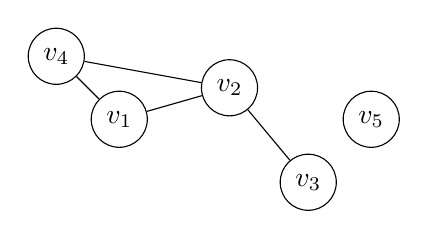
\begin{tikzpicture}[scale=0.8,mynode/.style=draw,circle]
\node[mynode] (v1) at (0,0) {$v_1$};
\node[mynode] (v2) at (1.75,0.5) {$v_2$};
\node[mynode] (v3) at (3,-1) {$v_3$};
\node[mynode] (v4) at (-1,1) {$v_4$};
\node[mynode] (v5) at (4,0) {$v_5$};
\draw (v1) -- (v2);
\draw (v1) -- (v4);
\draw (v2) -- (v4);
\draw (v2) -- (v3);
\draw (v5);
\end{tikzpicture}


\end{column}

\begin{column}{0.35\textwidth}
\scriptsize
\underline{\it Rótulos\/}\\
$v_1$ -- Brasil\\
$v_2$ -- Argentina\\
$v_3$ -- Chile \\
$v_4$ -- Paraguai \\
$v_5$ -- Equador
\end{column}

\end{columns}

\end{frame}

\begin{frame}{Matriz de adjacências}

\begin{columns}
\begin{column}{0.6\textwidth}
	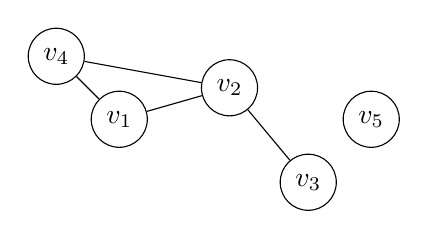
\begin{tikzpicture}[scale=0.8,mynode/.style=draw,circle]
\node[mynode] (v1) at (0,0) {$v_1$};
\node[mynode] (v2) at (1.75,0.5) {$v_2$};
\node[mynode] (v3) at (3,-1) {$v_3$};
\node[mynode] (v4) at (-1,1) {$v_4$};
\node[mynode] (v5) at (4,0) {$v_5$};
\draw (v1) -- (v2);
\draw (v1) -- (v4);
\draw (v2) -- (v4);
\draw (v2) -- (v3);
\draw (v5);
\end{tikzpicture}


\end{column}
\begin{column}{0.4\textwidth}
	$v_1  v_2  v_3  v_4  v_5$ \\
 	0  1  0  1  0 \\
 	1  0  1  1  0 \\
 	0  1  0  0  0 \\
 	1  1  0  0  0 \\
 	0  0  0  0  0
\end{column}
\end{columns}

\end{frame}


\begin{frame}{Representação de grafos usando lista ligada}

\begin{columns}
\begin{column}{0.375\textwidth}
	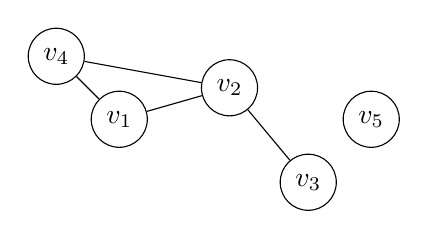
\begin{tikzpicture}[scale=0.8,mynode/.style=draw,circle]
\node[mynode] (v1) at (0,0) {$v_1$};
\node[mynode] (v2) at (1.75,0.5) {$v_2$};
\node[mynode] (v3) at (3,-1) {$v_3$};
\node[mynode] (v4) at (-1,1) {$v_4$};
\node[mynode] (v5) at (4,0) {$v_5$};
\draw (v1) -- (v2);
\draw (v1) -- (v4);
\draw (v2) -- (v4);
\draw (v2) -- (v3);
\draw (v5);
\end{tikzpicture}


\end{column}
\begin{column}{0.6\textwidth}
	\includegraphics[scale=0.275]{img/graph.png}
\end{column}
\end{columns}

\end{frame}


\begin{frame}{Grafos direcionados ou dígrafos: Definição}

\begin{block}{Informal}
Grafo direcionado ou dígrafo $G^\rightarrow$ é formado:
\begin{itemize}
\item Conjunto finito de vértices $V$;
\item Relação $R$ em $V$ entre os pares ordenados de arcos;
\item O conjunto de pares ordenados de arcos em $R$ é denotado por $E$.
\end{itemize}
\end{block}

\begin{block}{Formal}
$G^\rightarrow = (V, E)$ \\
$\{v \in V : v \notin \emptyset\}$ \\
$\{ (u, v) \in R : (u, v) \in E \land \{u, v\} \in V\}$ \\
\end{block}

\end{frame}


\begin{frame}{Dígrafo: exemplo}

\begin{block}{Representação simbólica}
\scriptsize
$G = (V, E)$

$V = \{v_1, v_2, v_3, v_4, v_5\}$
$R = \{(v_1, v_2), (v_2, v_3), (v_2, v_4), (v_4, v_1)\}$
$E  = \{(v_1, v_2), (v_4, v_1), (v_2, v_3), (v_2, v_4)\}$
     
\end{block}

\end{frame}

\begin{frame}{Dígrafo: Representação pictórica}

\begin{columns}
\begin{column}{0.6\textwidth}
\input{img/adigraph}
\end{column}

\begin{column}{0.35\textwidth}
\scriptsize
\underline{\it Rótulos\/}\\
TODO
\end{column}

\end{columns}

\end{frame}

\begin{frame}{Representação usando matriz de adjacências}

\begin{columns}
\begin{column}{0.6\textwidth}
\input{img/adigraph}
\end{column}

\begin{column}{0.4\textwidth}
$ v_1  v_2  v_3  v_4  v_5$ \\
 0  1  0  0  0 \\
 0  0  0  0  0 \\
 0  1  0  0  0 \\
 1  1  0  0  0 \\
 0  0  0  0  0 \\
\end{column}
\end{columns}

\end{frame}

\begin{frame}{Representação usando lista ligada}

\begin{columns}
\begin{column}{0.4\textwidth}
\input{img/adigraph}
\end{column}
\begin{column}{0.6\textwidth}
 \includegraphics[scale=0.35]{img/digraph.png}
\end{column}
\end{columns}

\end{frame}

\end{document}
